%% Metadaten
\begin{filecontents}{\jobname.xmpdata}
    \Title{Praxisnahe Anwendung der User-Centered Design Prinzipien: Neuentwicklung des Ethikantrag-Tools der Forschungsethik-Kommission der Fachhochschule Vorarlberg}
    \Author{Dominic Luidold, BSc}
    \Language{de-AT}
    \Keywords{TODO}
\end{filecontents}

\documentclass[a4paper,12pt,twoside]{scrreprt}
% Autor der Vorlage: Klaus Rheinberger, FH Vorarlberg, 2017-02-20

%% Pakete
% Dokumenteneigenschaften
\usepackage[ngerman]{babel}                 % Deutsche Sprachanpassungen
\usepackage[T1]{fontenc}                    % Silbentrennung bei Sonderzeichen
\usepackage[bindingoffset=8mm]{geometry}    % Bindeverlust von 8mm einbeziehen
\usepackage{minted}                         % Code Highlighting/Import
\usepackage[a-3b,mathxmp]{pdfx}[2018/12/22] % PDF/A
\usepackage{setspace}                       % Zeilenabstand

% Bilder
\usepackage{graphicx} % Bilder einbinden
\usepackage{wrapfig}  % Bilder positionieren

% Zitate & Verweise, Sonstiges
\usepackage[nohyperlinks]{acronym}  % Abkürzungsverzeichnis
\usepackage{caption}                % Abbildungslegenden
\usepackage{csquotes}               % Anführungszeichen und Zitieren
\usepackage[
    style=ieee,
    backend=biber
]{biblatex}                         % Literaturverweise
\usepackage{xcolor}                 % Farbige Hervorhebungen

%% Einstellungen
\addbibresource{references.bib}
\onehalfspacing
\setcounter{secnumdepth}{4} % Nummerierungstiefe
\setcounter{tocdepth}{3}    % Gliederungstiefe Inhaltsverzeichnis

%% Dokument
\begin{document}

% Titelblatt
\pagenumbering{roman}

\begin{titlepage}
    \begin{flushright}
    
\includegraphics[width=0.4\linewidth]{images/FHV_FHV-Logo.png}
    \end{flushright}
    \vspace{1cm}

    \begin{flushleft}
    \section*{Praxisnahe Anwendung der User-Centered Design Prinzipien}
    \subsection*{Neuentwicklung des Ethikantrag-Tools der Forschungsethik-Kommission der Fachhochschule Vorarlberg}
    \vspace{1cm}

    Masterarbeit\\
    zur Erlangung des akademischen Grades
    \vspace{0.5cm}

    \textbf{Master of Science in Engineering (MSc)}

    \vspace{1cm}
    Fachhochschule Vorarlberg\newline
    Informatik Master

    \vspace{0.5cm}

    Betreut von\newline
    Karin Trommelschläger, MSc

    \vspace{0.5cm}

    Vorgelegt von\newline
    Dominic Luidold, BSc\newline
    Dornbirn, [Monat Jahr]
    \end{flushleft}
\end{titlepage}

% Widmung
\newpage
\section*{Widmung}
\label{sec:widmung}

\colorbox{yellow}{TODO - Widmung}

% Abstract [DE]
\newpage
\section*{Kurzreferat}
\label{sec:abstract-de}

\subsection*{Titel [DE]}

\colorbox{yellow}{TODO - Kurzreferat}

% Abstract [EN]
\newpage
\section*{Abstract}
\label{sec:abstract-en}

\subsection*{Titel [EN]}

\colorbox{yellow}{TODO - Abstract}

% Inhaltsverzeichnis
\cleardoublepage
\tableofcontents

% Abbildungsverzeichnis
\clearpage
\phantomsection
\addcontentsline{toc}{chapter}{Abbildungsverzeichnis}
\listoffigures

% Abkürzungsverzeichnis
\clearpage
\phantomsection
\addcontentsline{toc}{chapter}{Abkürzungsverzeichnis}
\chapter*{Abkürzungsverzeichnis}

\begin{acronym}
    \acro{ecs}[ECS]{Ethic Commission System}
    \acro{fhv}[FHV]{Fachhochschule Vorarlberg}
    \acro{föe}[FÖE]{Forum Österreichischer Ethikkommissionen}
    \acro{ieb}[IEB]{Institutionelle Ethikboard der Fachhochschule Gesundheitsberufe OÖ}
    \acro{poc}[PoC]{Proof of Concept}
    \acro{ux}[UX]{User Experience}
\end{acronym}

% Inhalt
\cleardoublepage
\pagenumbering{arabic}

\chapter{Einleitung}
\label{chap:einleitung}

Die vorliegende Masterarbeit beschäftigt sich mit dem Erstellen und Einreichen von Ethikanträgen, die bei der Forschungsethik-Kommission der Fachhochschule Vorarlberg\footnote{\href{https://www.fhv.at/forschung/forschungsethik-kommission/}{Forschungsethik-Kommission: Analyse von Forschungstätigkeiten und deren ethischer Grundsatzfragen (\url{https://www.fhv.at/forschung/forschungsethik-kommission/)}}} eingereicht werden können. Ziel dieser Arbeit ist es, Lösungsvorschläge auszuarbeiten, die das auf Word-Dokumentenvorlagen aufbauende System langfristig ablösen können.

\section{Motivation}
\label{sec:motivation}

An der Fachhochschule Vorarlberg finden in einer Forschungsgruppe und fünf verschiedenen Forschungszentren, darunter beispielsweise die Forschungszentren \enquote{Nutzerzentrierte Technologien} und \enquote{Business Informatics}, Forschung und Entwicklung mit vermehrtem Augenmerk auf regionaler Zusammenarbeit aber auch internationaler Kooperationen statt.\cite{fachhochschule_vorarlberg_gmbh_forschung_2021} Um etwaige ethische Aspekte von Forschungsprojekten oder Entwicklungsarbeiten abwägen zu können, stehen den genannten Forschungseinrichtungen sowie allen Master-Studierenden der Fachhochschule Vorarlberg (im Rahmen ihres Kontextstudiums\footnote{\href{https://www.fhv.at/studium/kontextstudium-der-masterstudien/}{Kontextstudium der Masterstudien (\url{https://www.fhv.at/studium/kontextstudium-der-masterstudien/)}}} oder der Masterarbeit) eine direkt an der Fachhochschule ansässige Forschungsethik-Kommission zur Verfügung. Die Kommission gibt auf Antrag eine Stellungnahme beziehungsweise ein Votum zu einer geplanten wissenschaftlichen Untersuchung oder einem Forschungsvorhaben ab. Das Hauptaugenmerk der Ethikkommission liegt hierbei vor allem auf der Beurteilung von Projekten und Entwicklungsarbeiten, bei denen Menschen beteiligt sind, untersucht werden oder bei denen Folgen für die Beteiligten zu erwarten sind. Der bei einem entsprechenden Forschungsvorhaben einzureichende Antrag wird, zum Zeitpunkt dieser Arbeit im Sommersemester 2023, mittels einer Word-Dokumentenvorlage abgebildet. Um ein Votum von der Forschungsethik-Kommission zu erhalten, muss -- vereinfacht zusammengefasst -- die entsprechende Vorlage ausgefüllt und per E-Mail an den Vorsitz der Kommission gesendet werden.\cite{fachhochschule_vorarlberg_gmbh_forschungsethik-kommission_2021}

\medskip

Aufgrund von Feedback von Mitgliedern der Kommission und durch Anregungen von ehemaligen Antragssteller:innen ergibt sich für die Forschungsethik-Kommission die Situation, dass der gesamte Prozess von der Erstellung hin bis zum Einreichen eines Ethikantrages überdacht werden soll -- vor allem auch in Hinblick auf die technischen und inhaltlichen Limitierungen der Word-Dokumentenvorlage. Die Motivation dieser Arbeit ergibt sich daher aus dem Umstand, dass das aktuelle System rund um die zu behandelnden Ethikanträge nicht mehr den Anforderungen und Wünschen der Foschungsethik-Kommission der Fachhochschule Vorarlberg entspricht. Als weitere Motivation dient der Ausblick darauf, dass die grundlegende Analyse des Prozesses sowie der Vorschlag möglicher Lösungsansätze beziehungsweise eine etwaige Umsetzung eines Prototyps den Grundstein für weitere Schritte in Richtung einer angepassten und nutzerzentrierten Herangehensweise für alle Beteiligten bereitstellen kann. 

\section{Zielsetzung}
\label{sec:zielsetzung}

Die Zielsetzung dieser Masterarbeit lässt sich in zwei verschiedene Kategorien einteilen:
\begin{itemize}
    \item \textit{Unmittelbare Ziele} als direkte Resultate der Masterarbeit
    \item \textit{Langfristige Ergebnisse} aufbauend auf den unmittelbaren Zielen, jedoch außerhalb des Rahmens dieser Masterarbeit
\end{itemize}

\subsection{Unmittelbare Ziele}
\label{sub-sec:unmittelbare-ziele}

Die Masterarbeit hat das grundlegende Ziel, den aktuellen Prozess des Erstellens und Einreichens eines Ethikantrages für die Forschungsethik-Kommission der Fachhochschule Vorarlberg zu analysieren, um die bestehenden Probleme und Schwachstellen detailliert zu identifizieren und festzustellen. Durch die gewonnenen Informationen sowie die Erkenntnisse aus einer ebenfalls detailliert durchgeführten Ist-Analyse anderer Systeme soll ein Lösungsansatz entwickelt werden, dessen Umsetzung sich an den Prinzipien des Human-Centered Design orientiert.

Der angestrebte Lösungsansatz, in Form eines \ac{poc} anhand eines Prototyps mit grundlegenden Funktionen, soll während der Konzeptions- und Implementierungsphase evaluiert werden, um sicherzustellen, dass die Bedürfnisse der Antragssteller:innen und der Forschungsethik-Kommission zielgerichtet erfüllt werden. Der \ac{poc} beziehungsweise Prototyp kann und soll als Grundlage für weitere Entwicklungen und Optimierungen dienen können.

Ein weiterer wichtiger Aspekt und somit Ziel der Masterarbeit ist die Auseinandersetzung mit den Anforderungen an die Sicherheit und den Datenschutz im Prozess des Erstellens und Einreichens eines Ethikantrages. Dieser Aspekt soll in die Analyse und die Entwicklung von Lösungsansätzen einbezogen werden, um sicherzustellen, dass der neue Prozess nicht nur benutzerfreundlicher, sondern auch auf die Aspekte der Datensicherheit und Datenschutz abgestimmt ist.

\subsection{Langfristige Ergebnisse}
\label{sub-sec:langfristige-ergebnisse}

Neben den in Abschnitt \ref{sub-sec:unmittelbare-ziele} auf Seite \pageref{sub-sec:unmittelbare-ziele} definierten unmittelbaren Zielen können weitere, längerfristige Ergebnisse abgesteckt werden, die wiederum als Kriterium zur Erfolgsmessung dieser Masterarbeit herangezogen werden können.

Als wichtigstes Ergebnis zählt vor allem, dass die gewonnenen Erkenntnisse für die weiterführende Entwicklung und Optimierung des Prozesses, und bestenfalls des Prototyps, von Personen aufgegriffen und verwendet werden können, die nicht direkt an der Ausarbeitung der Arbeit beteiligt waren. Voraussetzung dafür ist das Ergebnis des \ac{poc} am Ende der Ausarbeitung dieser Masterarbeit. Sollte der Prototyp anhand des Feedbacks der Forschungsethik-Kommission sowie beteiligter Antragssteller:innen als vielversprechend beurteilt werden, kann die aktuelle Word-Dokumentenvorlage als langfristiges Ergebnis durch den entwickelten Lösungsansatz abgelöst werden.

\medskip

Unabhängig davon lassen sich weitere Ergebnisse definieren, die aufgrund der zeitlichen Komponente außerhalb des Rahmens dieser Masterarbeit sowohl betrachtet werden sollen als auch müssen:
\begin{itemize}
    \item Ein verbesserter und anwenderfreundlicherer Prozess des Erstellens und Einreichens eines Ethikantrages für die Forschungsethik-Kommission an der Fachhochschule Vorarlberg wurde geschaffen.
    \item Eine höhere Transparenz und Nachvollziehbarkeit des Prozesses für alle Beteiligten sowie eine verbesserte Zusammenarbeit zwischen der Forschungsethik-Kommission und den Forschenden beziehungsweise Master-Studierenden ist bemerkbar.
    \item Es lässt sich eine höhere Beteiligung der Betroffenen am Prozess realisieren, was zu einer höheren Berücksichtigung der Perspektiven aller Beteiligter führt.
    \item Die Verwendung von angemessenen Technologien hat den Prozess weitestgehend automatisiert und vereinfacht sowie die Datensicherheit und den Datenschutz gewährleistet.
\end{itemize}

\section{Frage-/Problemstellung}
\label{sec:frage-problemstellung}

Aufgrund der gegebenen Ausgangssituation ergibt sich die Frage, wie der Prozess des Erstellens und Einreichens eines Ethikantrages für die Forschungsethik-Kommission an der Fachhochschule Vorarlberg sinnvollerweise neu gestaltet und potenziell umgesetzt werden kann. Hauptaugenmerk soll dabei vor allem auf dem Aspekt einer verbesserten Usability beziehungsweise auf der Anwendung der Prinzipien des Human/User-Centered Design liegen.

Die Frage- beziehungsweise Problemstellung weitet sich zudem dahingehend aus, wie verhindert werden kann, dass die durch diese Masterarbeit erarbeiteten Lösungsansätze lediglich einer Eins-zu-Eins Umsetzung der Word-Dokumentenvorlage entsprechen. Hauptaugenmerk der Arbeit soll weiterhin sein, dass eine entsprechend tiefe Einarbeitung in die Materie und in die Prinzipien des Human/User-Centered Designs möglich ist.

\medskip

Die in dieser Masterarbeit behandelten Frage- beziehungsweise Problemstellungen sehen daher wie folgt aus:
\begin{itemize}
    \item Wie kann eine Neuentwicklung des Systems beziehungsweise Tools zur Erstellung und Einreichung eines Ethikantrages für die Forschungsethik-Kommission der Fachhochschule Vorarlberg anhand der User-Centered Design Prinzipien aussehen?
    \item Wie kann die Beteiligung der Anwender:innen am Designprozess sichergestellt werden, um ihre Bedürfnisse und Erwartungen besser zu verstehen und zu berücksichtigen?
    \item Welche technischen Lösungen können eingesetzt werden, um den Prozess der Erstellung und Einreichung eines Ethikantrages zu vereinfachen und zu automatisieren?
    \item Wie kann sichergestellt werden, dass der Prozess der Erstellung und Einreichung eines Ethikantrages den Datenschutz- und Datensicherheitsanforderungen entspricht?
\end{itemize}

\section{Vorgehensweise}
\label{sec:vorgehensweise}

Um ein grundlegendes Verständnis über die Thematik sowie den bestehenden Ablauf eines Ethikantrages zu erlangen, wird zu Beginn der Arbeit auf den Aufgabenbereich und die Arbeitsweise der Forschungsethik-Kommission eingegangen sowie der aktuelle Prozess rund um das Erstellen und Einreichen von Ethikanträgen beleuchtet. Dabei werden mittels Fragebogen und gezielt geführter Interviews mit Mitgliedern der Forschungsethik-Kommission sowie potenziellen und ehemaligen Antragssteller:innen allfällige Schwachstellen aufgearbeitet und etwaige Wünsche für ein neues System erörtert.

Im Zuge der detaillierten Ist-Analyse des bestehenden Systems wird zudem die Herangehensweise von anderen Ethikkommissionen an Hochschulen und Universitäten innerhalb Österreichs analysiert, um Vergleichswerte zu sammeln und Unterschiede oder Gemeinsamkeiten definieren zu können. Ebenso werden Systeme evaluiert, die den Anforderungen der Forschungsethik-Kommission bereits entsprechen könnten, ohne jedoch einen spezifischen Bezug zur Erstellung und Einreichung von Ethikanträgen zu haben.

Bevor mit der praktischen Anwendung der User-Centered Design Prinzipien für die Neuentwicklung des Systems begonnen wird, wird das zugrundeliegende Konzept genauer erläutert. Dabei wird auf die Konzepte und Begrifflichkeiten eingegangen, die für die spezifischen Anwendungsfälle dieser Masterarbeit benötigt und angewendet werden.

\colorbox{yellow}{TODO - Auswertung, Endergebnis, Ausblick, etc.}

\section{Wissenschaftliche Komponente}
\label{sec:wissenschaftliche-komponente}

Die Anwendung der User-Centered Design Prinzipien und die nutzerzentrierte Umsetzung von Software-Lösungen sind an sich keine neuen oder unerforschten Themengebiete. Das an der Fachhochschule Vorarlberg ansässige Forschungszentrum \enquote{Nutzerzentrierte Technologien} beschäftigt sich etwa bereits seit 2004 mit der Schnittstelle zwischen Mensch und Technik in den unterschiedlichsten Gegebenheiten.\cite{fachhochschule_vorarlberg_gmbh_nutzerzentrierte_2021}

Diese Masterarbeit beschäftigt sich, wie in diesem Einleitungskapitel mehrfach ausgeführt, vor allem mit der Erstellung und Einreichung von Ethikanträgen. Der Fokus der Arbeit liegt dabei nicht nur auf der technischen Umsetzung und der Anwendung der User-Centered Design Prinzipien, sondern vor allem auf der breit gefassten Analyse des gesamten Prozesses. Diese Masterarbeit soll -- wie den langfristigen Ergebnissen in Kapitel \ref{sub-sec:langfristige-ergebnisse} auf Seite \pageref{sub-sec:langfristige-ergebnisse} zu entnehmen ist -- eine Verbesserung sowohl für die Forschungsethik-Kommission als auch etwaigen Antragssteller:innen bringen, um die allgemeine Beteiligung am Prozess, die Transparenz und schlussendlich die Anzahl an Ethikanträgen zu steigern.

Von Beginn an anzunehmen, dass lediglich die Word-Dokumentenvorlage und nicht anderweitige Gründe von der Einreichung eines Ethikantrages abhalten, wäre unangebracht. Die wissenschaftliche Komponente ergibt sich daher aus dem Versuch der Annäherung an die zugrundeliegenden Probleme, Stärken und Anforderungen des bestehenden Ethikantrag-Prozesses in Zusammenspiel mit einer gleichzeitigen Ausarbeitung einer technischen Lösung anhand nutzerzentrierter Prinzipien und dem User-Centered Design Ansatz.

\chapter{Analyse des bestehenden Prozesses}
\label{chap:analyse-bestehender-prozess}

\section{Objektive Analyse}

\section{Analyse Anhand von Interviews}

\section{Erfahrung aus eigener Einreichung}

\chapter{Analyse anderer Systeme}
\label{chap:analyse-anderer-systeme}

Um neben der Analyse des bestehenden Systems beziehungsweise Prozesses rund um die Word-Dokumentenvorlage Vergleichswerte sammeln zu können, werden weitere Systeme sowohl mit spezifischem Fokus auf Ethikanträgen als auch Systeme ohne direkten Bezug genauer betrachtet und Unterschiede sowie Gemeinsamkeiten herausgearbeitet.

Durch die breiter gefasste Erhebung zum Stand der Technik können so zusätzliche Herangehensweisen oder Anforderungen, die in der Analyse in Kapitel \ref{chap:analyse-bestehender-prozess} ab Seite \pageref{chap:analyse-anderer-systeme} nicht aufgegriffen werden konnten, abgedeckt werden. Ebenso kann dadurch eruiert werden, ob ein bestehendes System die Möglichkeit bietet, soweit an die Anforderungen der Forschungsethik-Kommission sowie der Antragssteller:innen angepasst werden zu können, als das eine gänzliche Neuentwicklung nicht mehr notwendig ist.

\section{Systeme mit Fokus auf Ethikanträgen}
\label{sec:systeme-mit-fokkus-ethikantrage}

\subsection{Vorlage des Forums Österreichischer Ethikkommissionen}
\label{sub-sec:vorlage-föe}

Das \ac{föe}\footnote{\href{https://me001ned.edis.at/ethikkommission/Forum/index.htm}{Forum Österreichischer Ethikkommissionen (\url{https://me001ned.edis.at/ethikkommission/Forum/)}}} ist ein freiwilliger Zusammenschluss von Ethikkommissionen in Österreich mit medizinischem Fokus und mit dem Hintergrund, einheitliche Arbeitsweisen und Formulare (für beispielsweise Meldungen, Anträge etc.) für österreichiche Ethikkommissionen zu schaffen.\cite{ethikkommission_der_medizinischen_universitat_graz_forum_2019}

Ähnlich zur Herangehensweise der Forschungsethik-Kommission der Fachhochschule Vorarlberg basieren die vom \ac{föe} bereitgestellten Unterlagen auf Dokumentenvorlagen im \texttt{.dot} beziehungsweise \texttt{.rtf} Dateiformat, wobei die Nutzung von Microsoft Word vom Forum explizit empfohlen wird. Neben dem zum Download angebotenen Antrag\footnote{\href{https://me001ned.edis.at/ethikkommission/Forum/Download/Files/Antr.dot}{Antragsformular in der Version 6.4 vom 12.06.2012 (\url{https://me001ned.edis.at/ethikkommission/Forum/Download/Files/Antr.dot})}} werden zusätzlich ein ausgefülltes Muster sowie Erläuterungen zum Antrag im \texttt{.pdf} Dateiformat beigelegt, welche erklären, wie die Vorlage geöffnet, ausgefüllt und gespeichert werden kann.\footnote{Die bereitgestellten Erläuterungen stammen aus dem Jahr 2004, weshalb diese aller Wahrscheinlichkeit nach so detailliert ausfallen (beispielsweise die Bezugnahme auf die Menüführung des damaligen \enquote{WinWord}).} \cite{ethikkommission_der_medizinischen_universitat_graz_download_2012}

Die in Abbildung \ref{fig:dokumentenvorlage-föe} auf Seite \pageref{fig:dokumentenvorlage-föe} dargestellte Dokumentenvorlage führt die Antragssteller:innen durch zwei verschiedene Teile (\enquote{Teil A} und \enquote{Teil B}), in denen unterschiedliche Angaben entweder in Freitext-Feldern oder in entsprechend anzukreuzenden Auswahl-Feldern getätigt und Fragen beantwortet werden können. Alle zu befüllenden Felder sind dabei mit einer eindeutigen Nummer gekennzeichnet und umfassen vom Projekttitel bis hin zur detaillierten Angabe von geplanten Therapie- und Diagnostikverfahren alle benötigten Informationen für die Bewertung der medizinischen Studie.

\begin{figure}[ht]
    \centering
    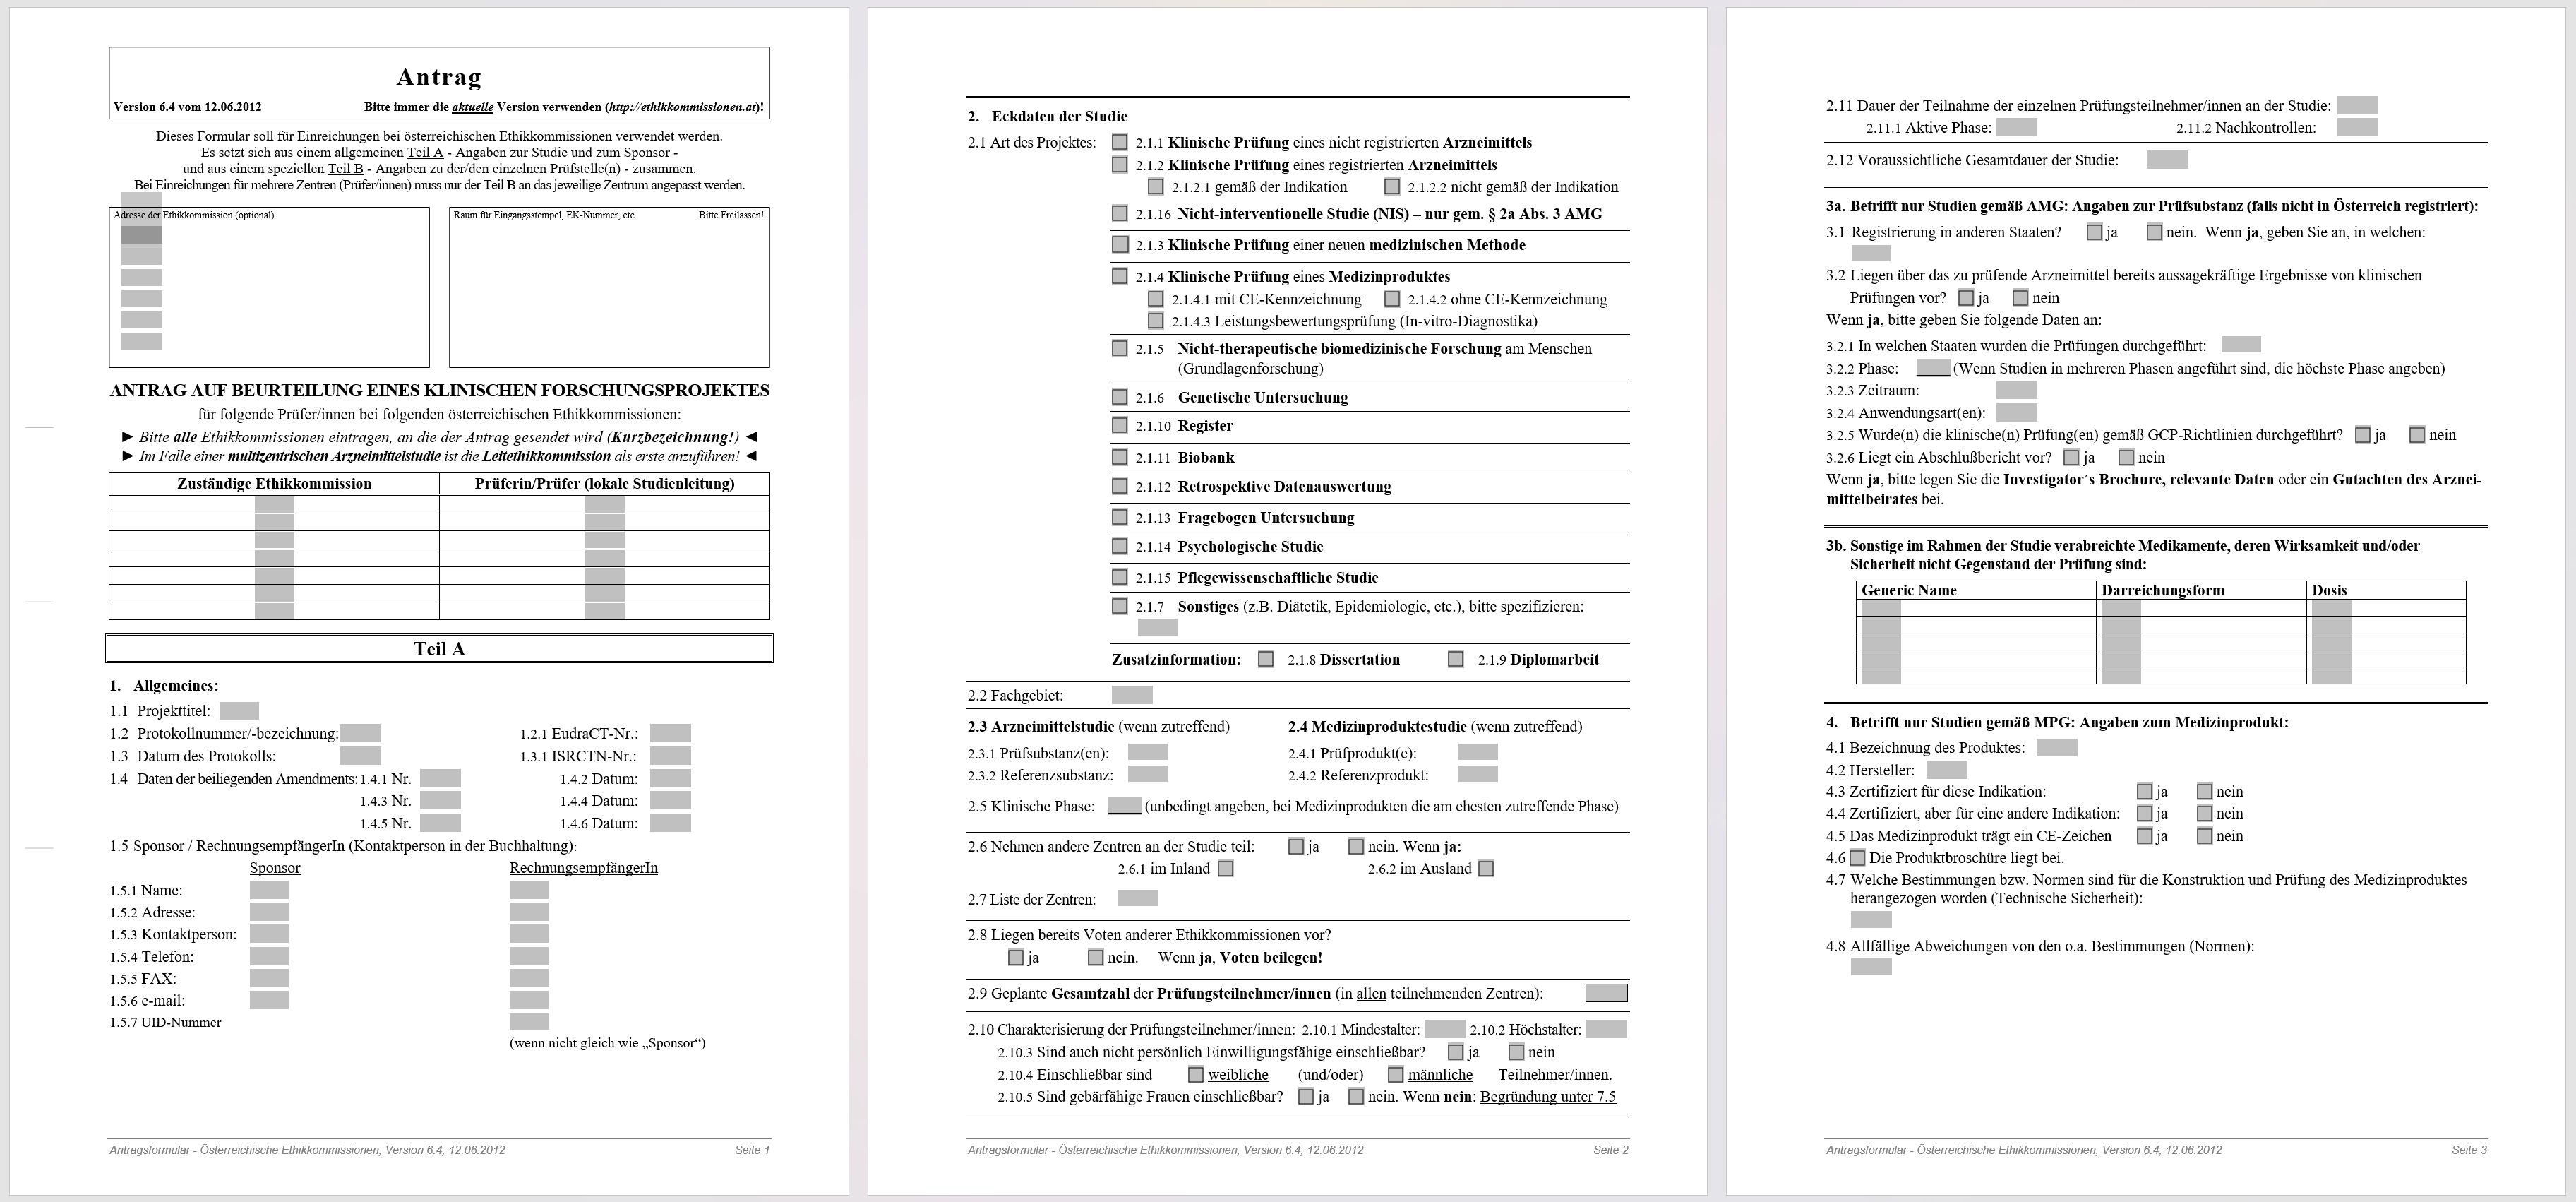
\includegraphics[scale=0.21]{thesis/images/Luidold_Word-Vorlage-Forum-Oesterreichischer-Ethikkommissionen.png}
    \caption[Screenshot der Word-Dokumentenvorlage des Forums Österreichischer Ethikkommissionen]{Screenshot des Antragsformulares auf Basis einer Word-Dokumentenvorlage des \ac{föe} (Quelle: eigene Abbildung)}
    \label{fig:dokumentenvorlage-föe}
\end{figure}

Bei der Durchsicht des Antrages fallen dabei folgende Punkte auf:
\begin{itemize}
    \item Die Vorlage enthält sowohl für die finale Beurteilung benötigte Informationen (die durch die Antragssteller:innen bereitgestellt werden) als auch Ausfüllhilfen und Hilfestellungen, die zwischen den einzelnen Punkten und Fragen eingebettet sind.
    \item Gewisse Tabellen (wie beispielsweise die Tabellen bei Punkt \enquote{6. Angaben zur durchzuführenden Therapie und Diagnostik} auf Seite 5 des Antrages) lassen nur eine gewisse Anzahl an Einträgen zu, ohne den Antragsstellenden die Möglichkeit zu geben, weitere Punkte hinzufügen zu können.
    \item Es stehen keinerlei Formatierungsmöglichkeiten zur Verfügung, um ausgefüllte Informationen beispielsweise mit kursiver oder farbig hinterlegter Schrift zu strukturieren. Alle getätigten Informationen sind automatisch in fetter Schrift angegeben, um sie von der Vorlage unterscheiden zu können.
\end{itemize}

Da das \ac{föe} keine eigene Ethikkommission darstellt, hängt der Prozess des Einreichens des erstellten und ausgefüllten Ethikantrages von der jeweiligen Ethikkommmission ab. Das Forum weißt jedoch darauf hin, dass es trotz der einheitlichen Formulare zusätzliche Anforderungen der Kommissionen geben kann oder das Formular gar nicht mehr in Form der zum Download angebotenen Dokumentenvorlage angenommen wird (für weitere Informationen siehe dazu Kapitel \ref{sub-sec:ecs} ab Seite \pageref{sub-sec:ecs}).\cite{ethikkommission_der_medizinischen_universitat_graz_download_2012}

Aufgrund des inhaltlichen Fokus des \acl{föe} auf medizinische Ethikkommissionen lassen sich aus dem Antrag nur bedingt Anforderungen für den in dieser Masterarbeit auszuarbeitenden Lösungsansatz ableiten. Vor auch aber deswegen nicht, da es sich ebenfalls um eine Dokumentenvorlage mit ähnlichen Problemen zur Vorlage der Forschungsethik-Kommission der Fachhochschule Vorarlberg handelt.

\subsection{Vorlage der FH Gesundheitsberufe OÖ}
\label{sub-cec:vorlage-fh-oö}

Das \ac{ieb}\footnote{\href{https://www.fh-gesundheitsberufe.at/f-e/institutionelles-ethikboard/}{Institutionelles Ethikboard der FH Gesundheitsberufe OÖ (\url{https://www.fh-gesundheitsberufe.at/f-e/institutionelles-ethikboard/})}} fokussiert sich auf die Überprüfung ethischer Aspekte bei eingereichten Forschungsprojekten an oder mit Menschen und darauf, ob eine zusätzliche Einreichung bei einer spezialisierten Ethikkommission notwendig ist.\cite{fh_gesundheitsberufe_oo_gmbh_institutionelles_2023}

Das \ac{ieb} greif dabei -- ebenso wie das \ac{föe} und die Forschungsethik-Kommission der Fachhochschule Vorarlberg -- auf eine Dokumentenvorlage\footnote{\href{https://www.fh-gesundheitsberufe.at/assets/files/IEB-Antragsformular_V1.00_21.09.2022.docx}{Antragsformular Version1 vom 21.09.2022 (\url{https://www.fh-gesundheitsberufe.at/assets/files/IEB-Antragsformular_V1.00_21.09.2022.docx)}}} im mit Microsoft Word kompatiblen \texttt{.docx} Dateiformat zurück. Diese Vorlage wird Antragssteller:innen zum Download angeboten und kann sowohl digital als auch in Printversion beim Ethikboard zur Begutachtung eingereicht werden. \cite{fh_gesundheitsberufe_oo_gmbh_einreichung_2023} Abbildung \ref{fig:dokumentenvorlage-ieb} auf Seite \pageref{fig:dokumentenvorlage-ieb} zeigt einen Ausschnitt des Dokumentes, welches mittels Freitext-Feldern und Kontrollkächsten vom Projekttitel bis hin zu detaillierten Fragen zum Studiendesign und Datenschutz abfragt.

\begin{figure}[ht]
    \centering
    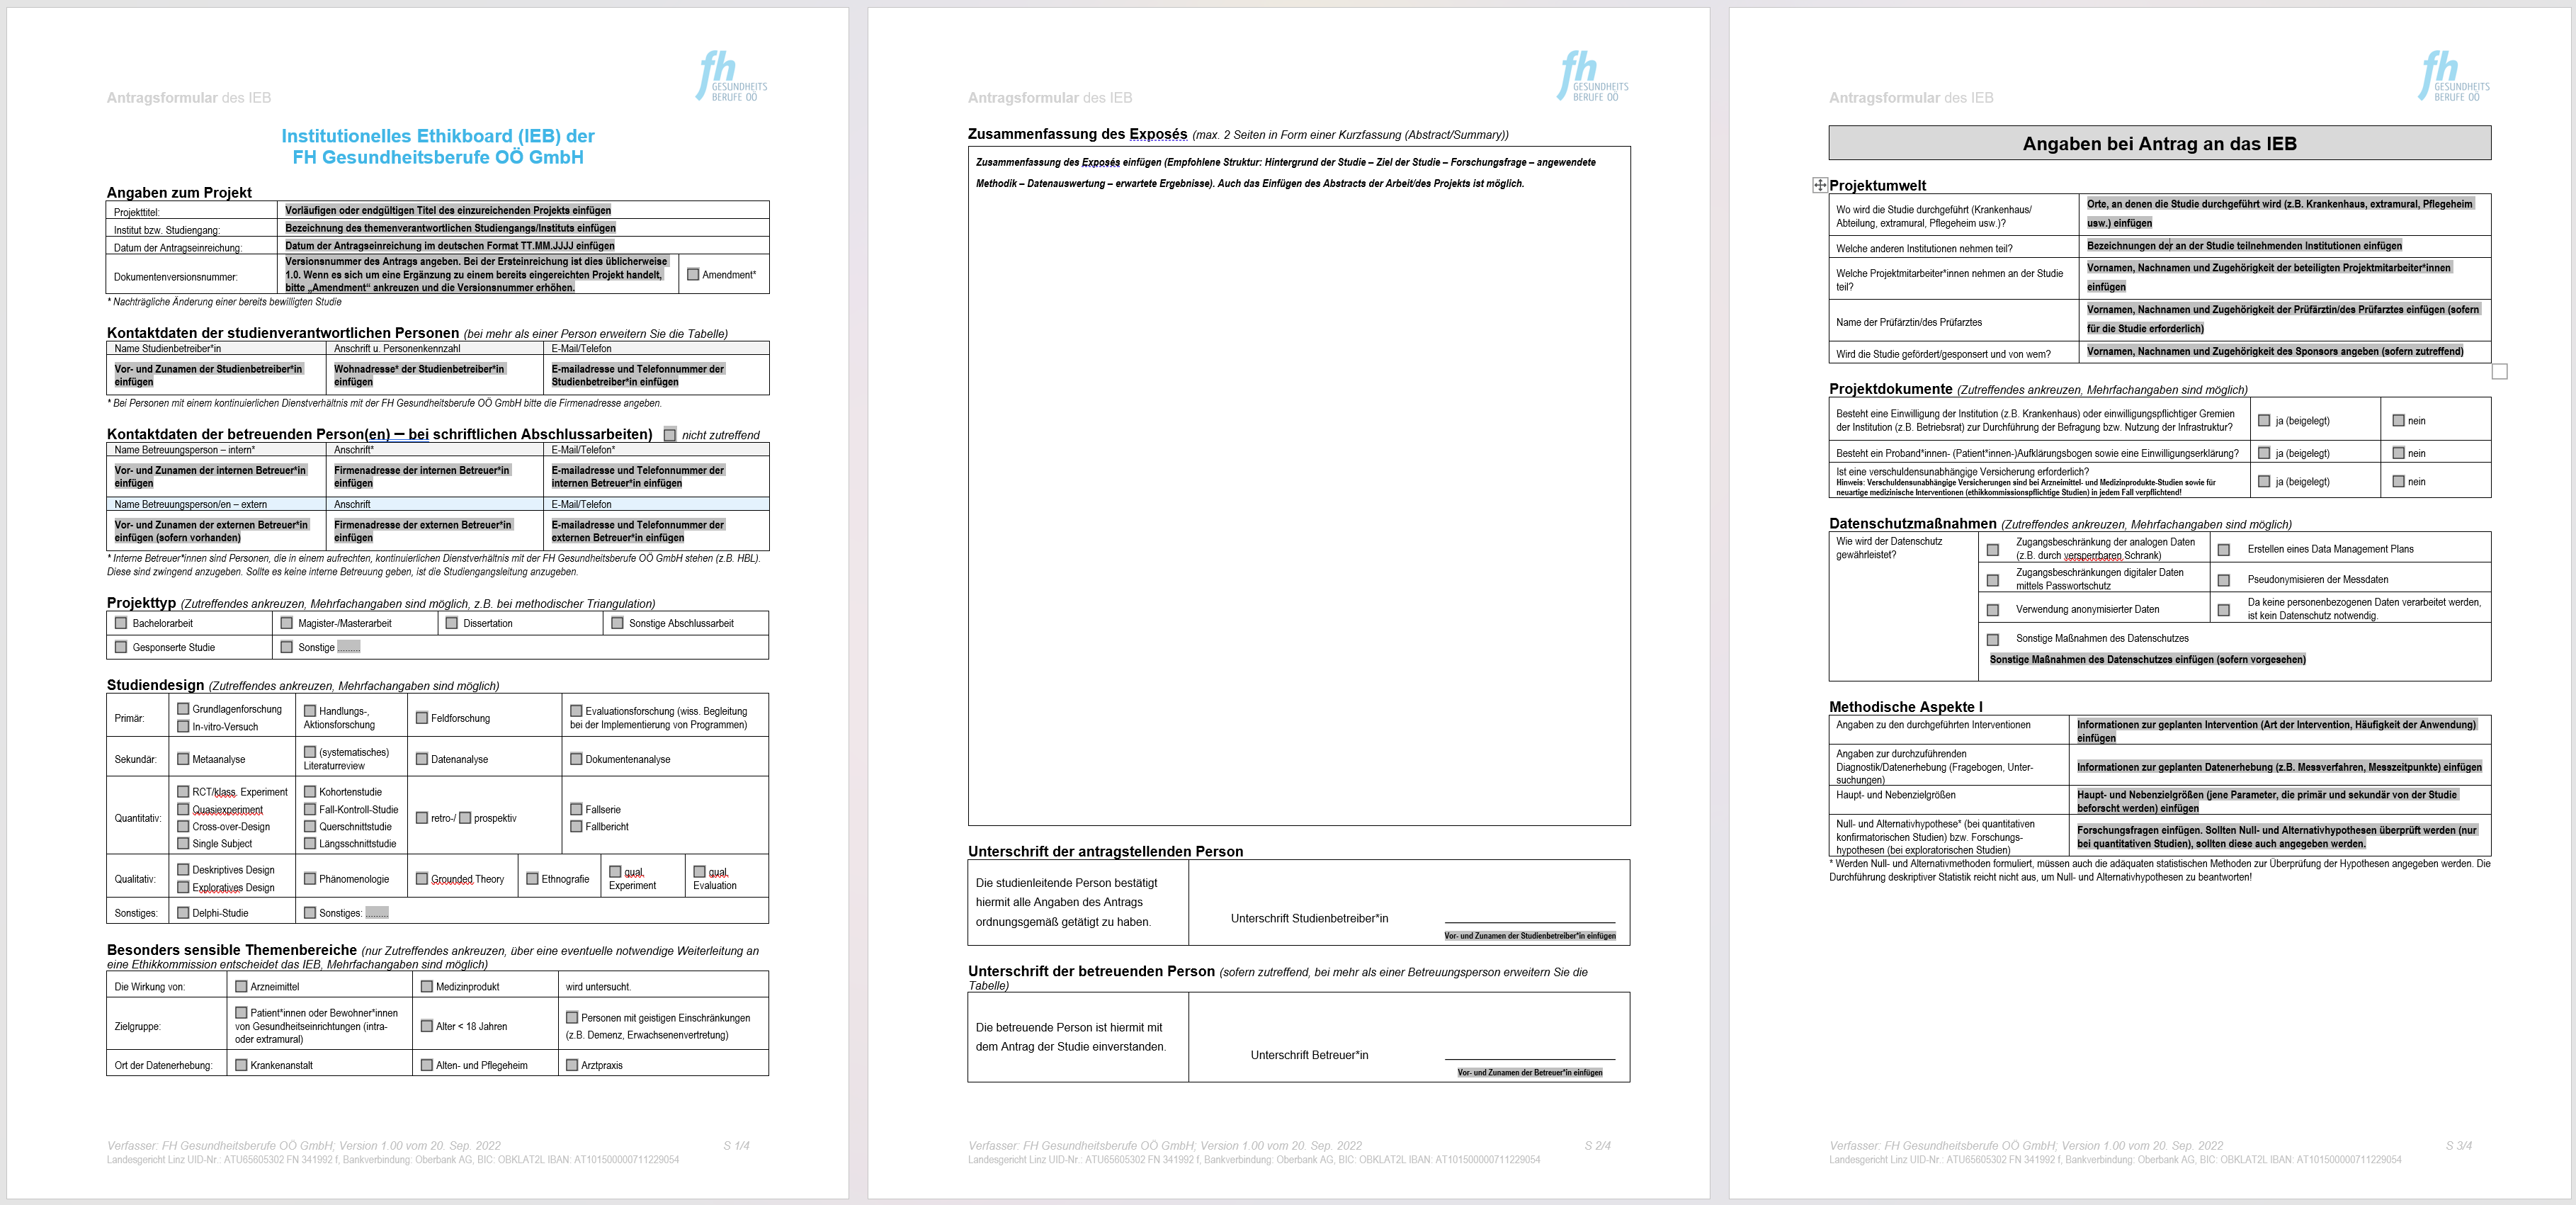
\includegraphics[scale=0.21]{thesis/images/Luidold_Word-Vorlage-IEB-FH-Gesundheitsberufe-OOE.png}
    \caption[Screenshot der Word-Dokumentenvorlage des Institutionellen Ethikboards der FH Gesundheitsberufe OÖ]{Screenshot des Antragsformulares auf Basis einer Word-Dokumentenvorlage des \ac{ieb} (Quelle: eigene Abbildung)}
    \label{fig:dokumentenvorlage-ieb}
\end{figure}

Bei der Durchsicht des Antrages fallen dabei folgende Punkte auf, die sich stellenweise von den Erkenntnissen zu der in Kapitel \ref{fig:dokumentenvorlage-föe} ab Seite \pageref{sub-sec:vorlage-föe} behandelten Antragsvorlage der \ac{föe} unterscheiden:
\begin{itemize}
    \item Die Vorlage enthält zusätzliche Punkte in Form von Ausfüllhilfen und Hilfestellungen, die die Antragsstellenden unterstützen sollen, nicht aber relevant für die finale Beurteilung sind.
    \item Konträr zur Dokumentenvorlage des \ac{föe} ist der Antrag keine strikte Umsetzung eines Formulars, sondern Antragsstellende können das Dokument und alle seine Elemente frei bearbeiten. Dadurch sind Anpassungen sowie auch das Hervorheben von Text mit beispielsweise unterstrichener, kursiver oder farbig hinterlegter Schrift möglich.
    \item Das Antragsformular weicht, trotz des Fokus der Fachhochschule und des \ac{ieb} auf medizinische Studien, sowohl vom Aufbau als auch vom abgefragten Inhalt 
\end{itemize}

\colorbox{yellow}{TODO - Rückmeldung IEB einbauen}

Der Prozess der Einreichung eines Ethikantrages wird vom \ac{ieb} in einen zweistufigen Prozess unterteilt, welcher detailliert in Abbildung \ref{fig:prozess-ethikantrag-ieb} auf Seite \pageref{fig:dokumentenvorlage-ieb} dargestellt wird. Nach initialer Überprüfung der Vollständigkeit wird der eingereichte Ethikantrag von zwei dem Ethikboard angehörigen Mitgliedern geprüft und entschieden, ob eine direkte Behandlung durch das \ac{ieb} möglich ist oder ob dieser bei einer spezialisierten Kommission eingereicht werden muss. Verläuft die weitere Prüfung positiv, kann dem Antrag entweder eine \enquote{Unbedenklichkeitsbescheinigung} ausgestellt werden oder es findet eine detaillierte Prüfung in einer Vollversammlung des \ac{ieb} statt, die bei Erfülllung etwaiger Auflagen in einem positiven Votum endet.\cite{fh_gesundheitsberufe_oo_gmbh_einreichung_2023}

\begin{figure}[ht]
    \centering
    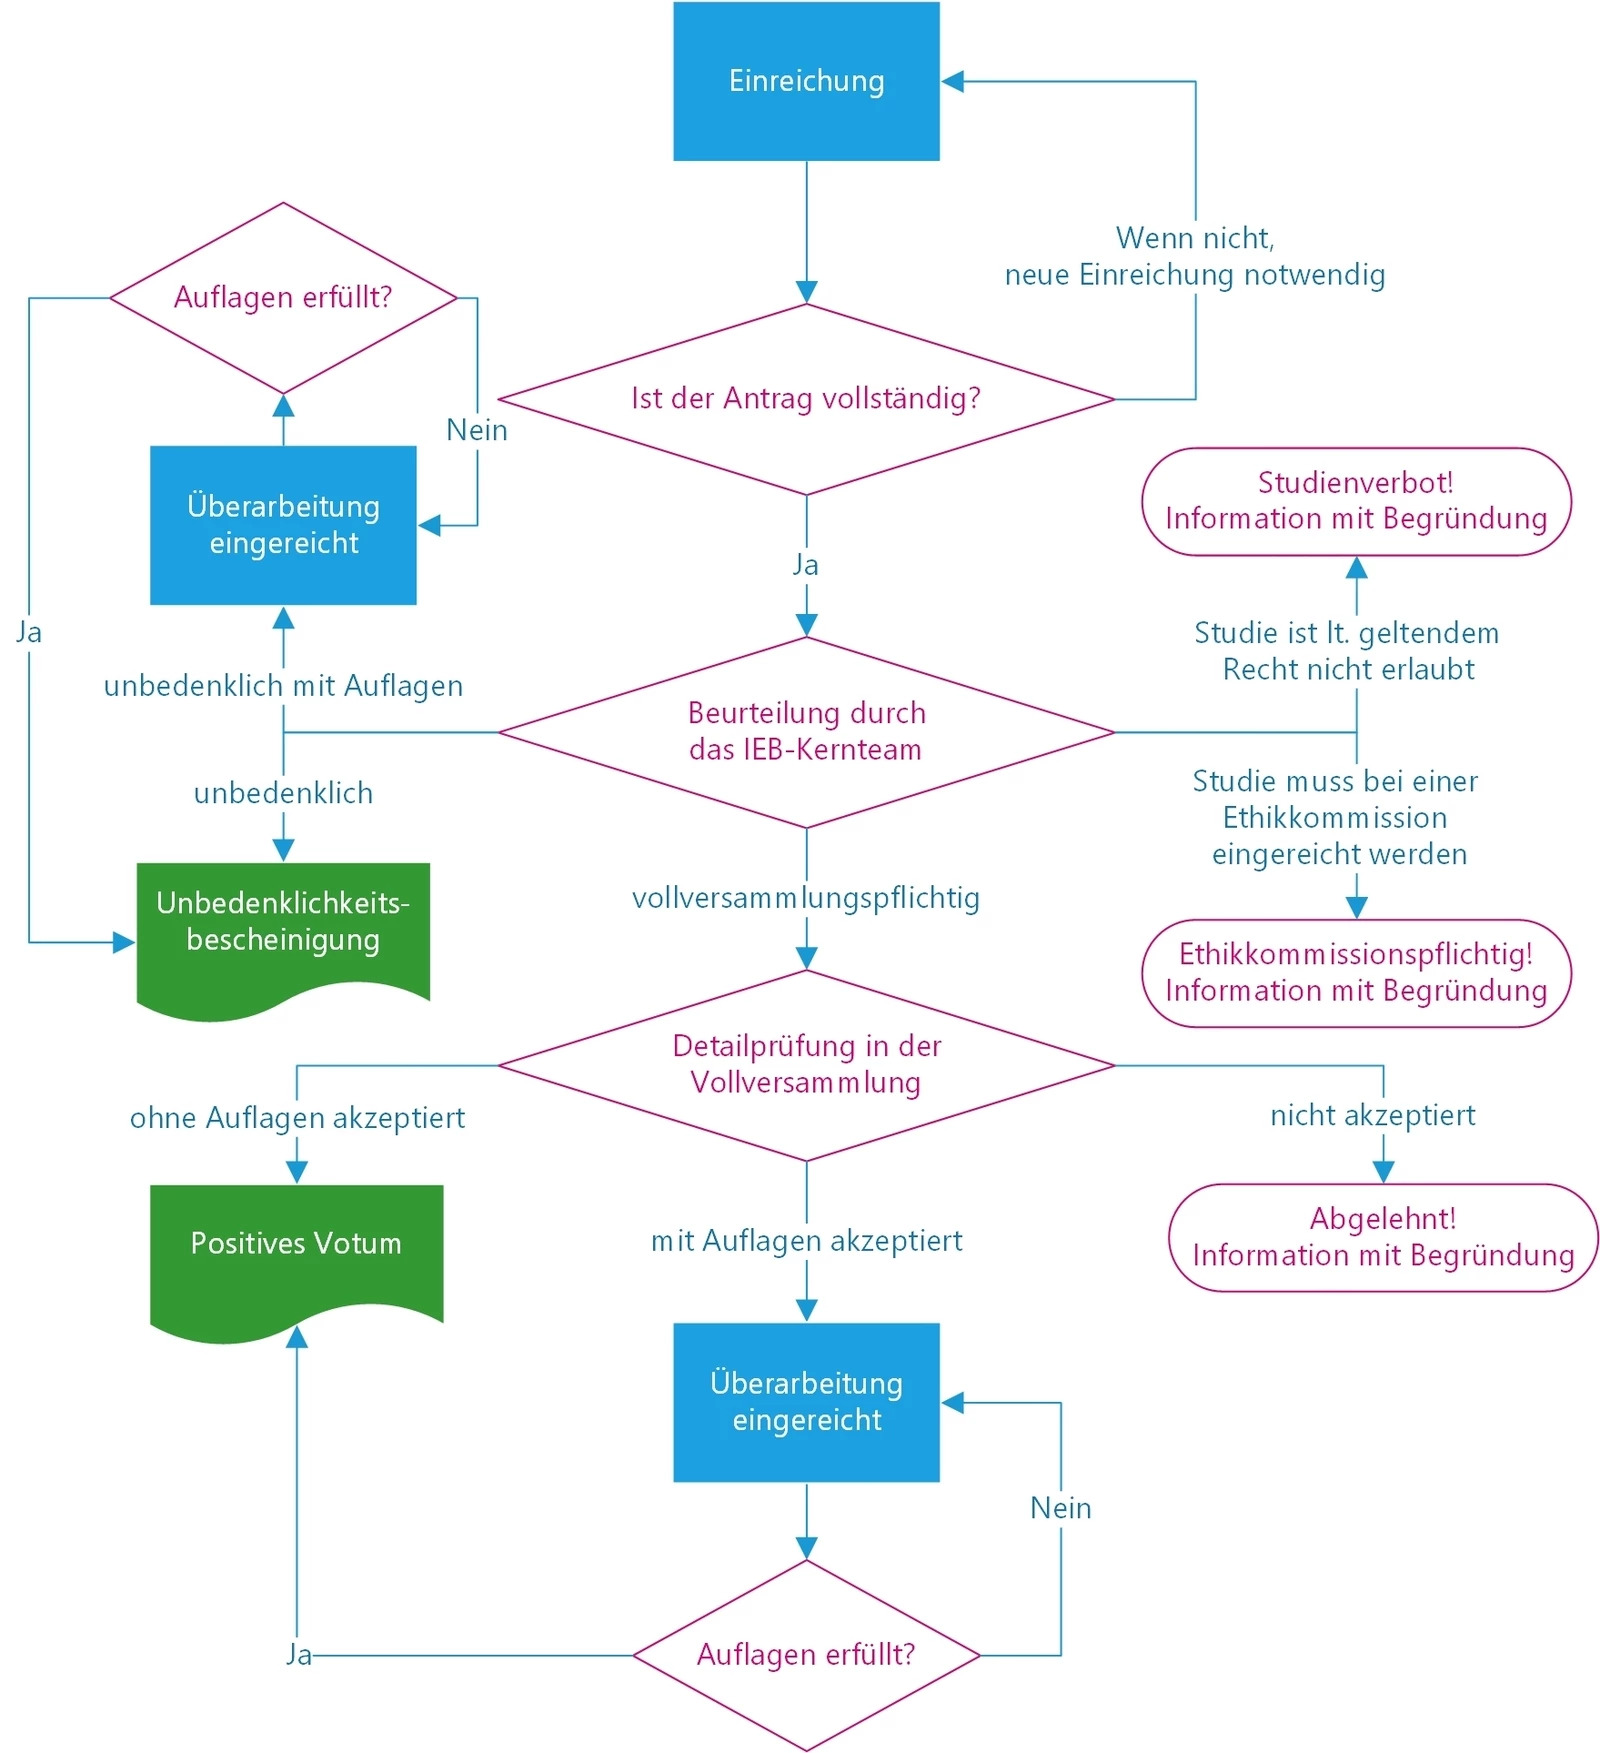
\includegraphics[scale=0.15]{thesis/images/FHGOOE_Prozess-Ethikantrag.jpg}
    \caption[Prozessdiagramm zur Einreichung eines Ethikantrages beim Institutionellen Ethikboard der FH Gesundheitsberufe OÖ]{Prozessdiagramm zur Einreichung eines Ethikantrages beim Institutionellen Ethikboard der FH Gesundheitsberufe OÖ \cite{fh_gesundheitsberufe_oo_gmbh_einreichung_2023}}
    \label{fig:prozess-ethikantrag-ieb}
\end{figure}

\colorbox{yellow}{TODO - Mögliche Ableitungen für eigene Umsetzung einbauen}

\subsection{Einreichplattform der FH Campus Wien}
\label{sub-sec:einreichplattform-fh-campus-wien}

todo

\subsection{Ethic Commission System (ECS)}
\label{sub-sec:ecs}

todo

\section{Systeme ohne konkreten Bezug}
\label{sec:systeme-ohne-bezug}

todo

% Literaturverzeichnis
\clearpage
\phantomsection
\addcontentsline{toc}{chapter}{Literaturverzeichnis}
\printbibliography

% Eidesstattliche Erklärung
\clearpage
\chapter*{Eidesstattliche Erklärung}
\addcontentsline{toc}{chapter}{Eidesstattliche Erklärung}
Ich erkläre hiermit an Eides statt, dass ich die vorliegende Masterarbeit selbstständig und ohne Benutzung anderer als der angegebenen Hilfsmittel angefertigt habe. Die aus fremden Quellen direkt oder indirekt übernommenen Stellen sind als solche kenntlich gemacht. Die Arbeit wurde bisher weder in gleicher noch in ähnlicher Form einer anderen Prüfungsbehörde vorgelegt und auch noch nicht veröffentlicht.

\vspace{5cm}
\noindent
Dornbirn, am [Tag. Monat Jahr anführen]\hfill Dominic Luidold, BSc

\end{document}
